
\hypertarget{working_shortcuts}{}
\section{Shortcuts customization}
\index{shortcuts}
\index{shortcuts!customization}

\begin{figure}[H]
  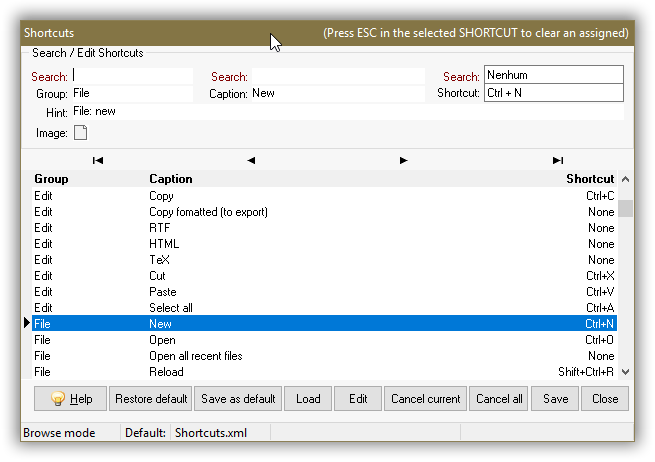
\includegraphics[scale=0.40]{./res/shortcuts_dlg.png}\\
  \caption{Shortcuts customization.}
  \label{fig:shortcuts_dlg_1}
\end{figure}

The \textit{Shortcuts customization}
(Figure \ref{fig:shortcuts_dlg_1})
allows the user to set the shortcuts related
to the application, it works together with the \textit{Editor keystrokes},
and allows for high level of customization.

The difference between \textit{Shortcuts} and \textit{Hotkeys (operational system)}
is that the former works only with the focus on Tinn-R, whereas hotkeys work
with the focus anywhere.

Read below a brief description of available buttons.

\begin{quote}
  \begin{footnotesize}
    \begin{description}
      \item[Restore default:]
        Restores the file \texttt{Shortcuts.xml} from the origin
        (InstallPath/data/data.zip). Any prior changes to the file
        \texttt{Shortcuts.xml} in use will be lost.
      \item[Save as default:]
        Opens the save dialog allowing to save the file. From this
        point, this file will be the new default shortcuts.
      \item[Load:]
        Opens the open dialog allowing to load a shortcut file. From this
        point on, this file will be the new default shortcuts.
      \item[Edit:]
        Sets the table in edition mode.
      \item[Cancel current:]
        Cancels any changes made to the current edition.
      \item[Cancel all:]
        Cancels all changes made to the database prior to \textit{Save}
        or \textit{Save as default}.
      \item[Save:]
        Saves to text file (XML) all changes made to the current table.
      \item[Close:]
        Closes the dialog. All changes not saved will be lost.
    \end{description}
  \end{footnotesize}
\end{quote}
